На рисунке() представлена схема программируемой логики.\par 
\begin{figure}[ht]
    \centering
    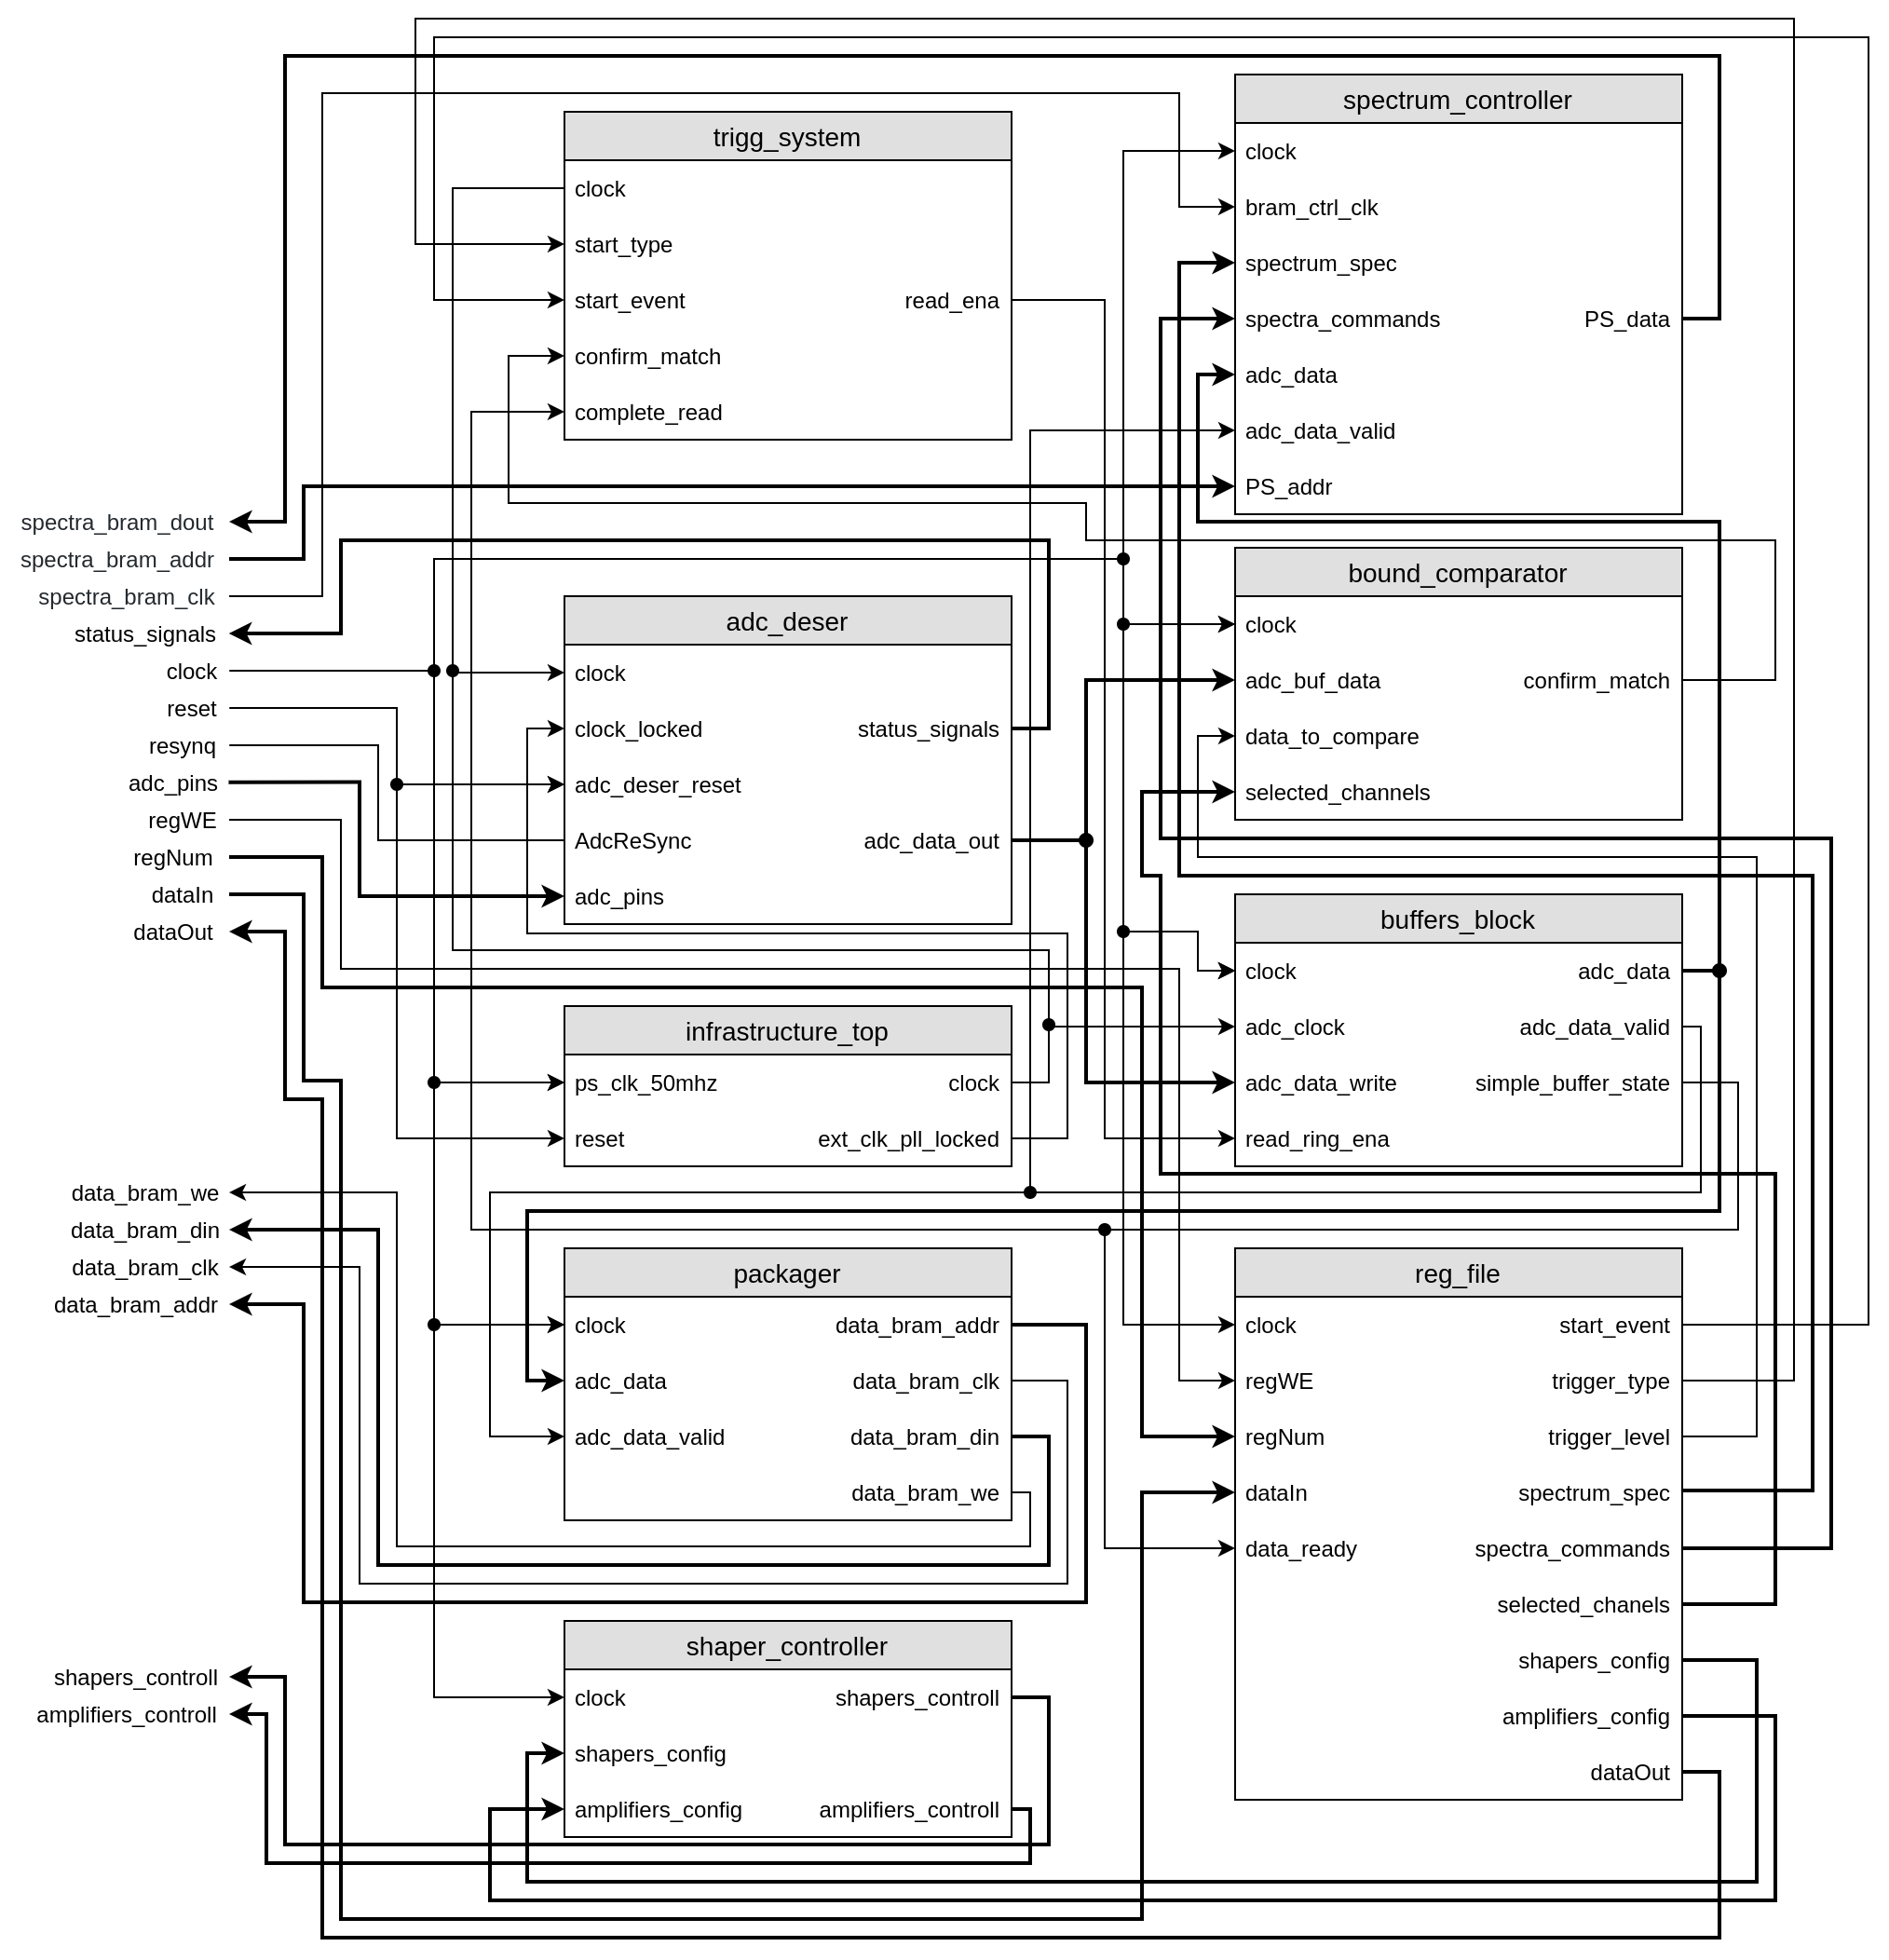
\includegraphics[width=1\linewidth]{PL_top.png}
    \caption{Блок-схема установки}
    \label{fig:mpr}
\end{figure}
Программируемая логика состоит из 9 блоков, краткое описание который представлено в таблице()\par
\begin{table}[h!]
    \caption{Блоки программируемой логики}
   % \begin{tabular}{|>{\centering\arraybackslash}p{0.45\textwidth}|>{\centering\arraybackslash}p{0.45\textwidth}|}
    \begin{tabular}{|p{0.45\textwidth}|p{0.5\textwidth}|}
        \hline
        Наименование блока & Описание \\
        \hline
        adc\_deser & Конвертирует упакованные последовательно данные АЦП в численные значения \\
        \hline
        infrastructure\_top & Обеспечивает тактовую частоту для некоторых модулей \\
        \hline
        buffers\_block & Буферизует входные данные \\
        \hline
        packager & Упаковывает данные и передаёт их в процессорную систему \\
        \hline
        shaper\_controller & Осуществляет управление формирователями сигналов \\
        \hline
        spectrum\_creator & Производит обработку данных для набора статистики \\
        \hline
        bound\_comparator & Выполняет сравнение входящих данных с заданными порогами \\
        \hline
        reg\_file & Реализует блок виртуальных регистров \\
        \hline
        trigg\_system & Генерирует сигнал для сохранения данных \\
        \hline
    \end{tabular}
\end{table}
\textbf{Десериализатор adc\_deser}\par
Одним из основных элементов стенда является АЦП AD-9253. Данный преобразователь работает на 125 МГц параллельно в 4-х каналах. Данные с разрешением 14 бит передаются по протоколу LVDS. Данный стандарт предполагает передачу информации в последовательно-упакованном виде по 2 каналам на каждый вход. На рисунке() представлена временная диаграмма работы АЦП.\par
\begin{figure}[ht]
    \centering
    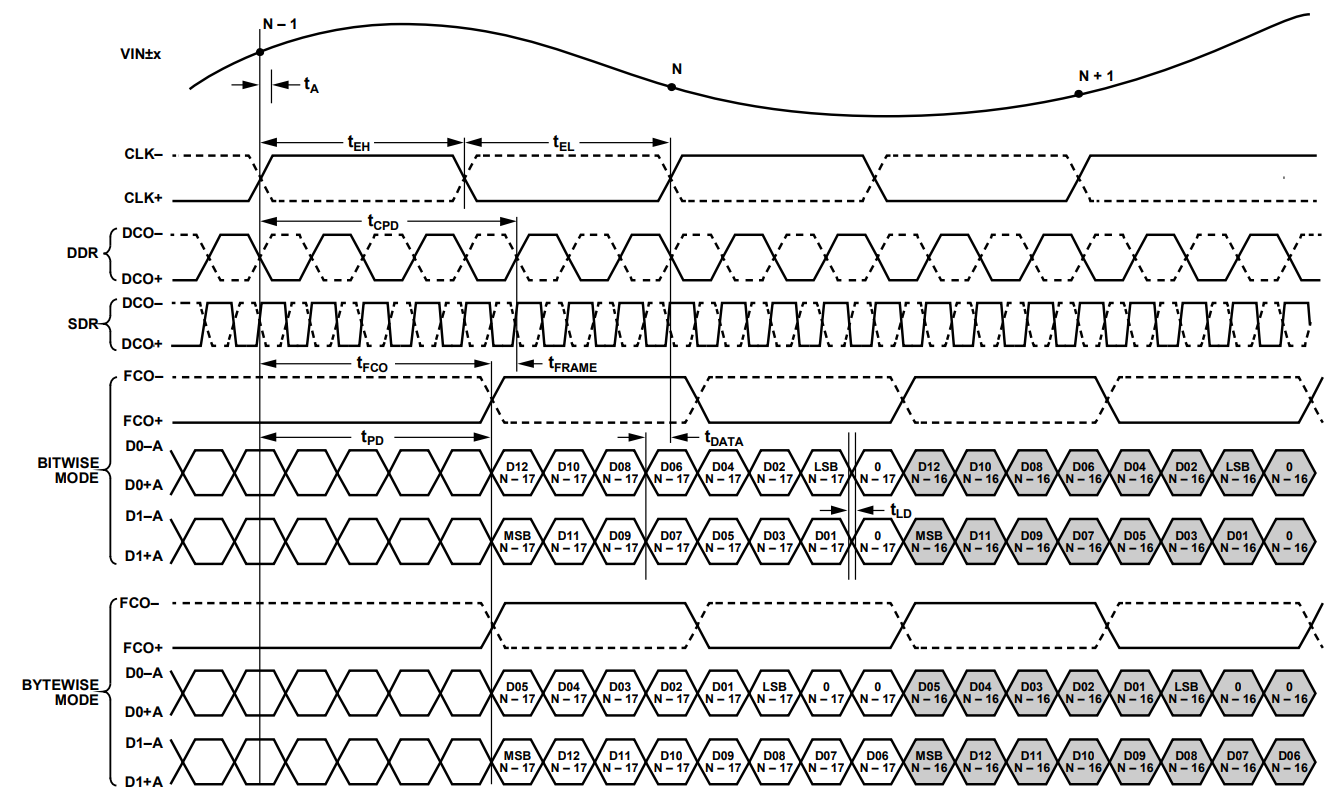
\includegraphics[width=1\linewidth]{ADC_time_diagram.png}
    \caption{Временная диаграмма работы АЦП}
    \label{fig:mpr}
\end{figure}
Каждый такт работы АЦП производится оцифровка входного аналогового сигнала. Как видно из временной диаграммы, полученные данные отправляются за 1 такт через 17 тактов после оцифровки по двум каналам. Предствляться они могут в одном из двух вариантов: побитовый (bitewise mode) и побайтовый (bytewise mode). Данные режимы отличаются последовательностью упаковки битов --- в разных каналах передаются либо четные и нечётные биты, либо младший и старший байты соответственно. В данной работе выбран побитовый режим, так как данные в таком виде проще обработать в программируемой логике.\par
Также в работе АЦП участвуют 2 вспомогательных сигнала --- кадровый, отвечающий за разделение набора бит на кадры оцифровки, и сигнал передачи данных, который размечает биты внутри каждого кадра.\par
Таким образом, возникает небходимость реализации модуля, осуществляющего конвертацию последовательности бит, поступающей из АЦП, в удобное для обработки численное значение. Так как процесс упаковки бит в определённую последовательность называется сериализацией, то обратную операцию можно назвать десериализаций, а соответствующий модуль --- десериализатором. Его сигналы изображены на рисунке()\par
\begin{figure}[ht]
    \centering
    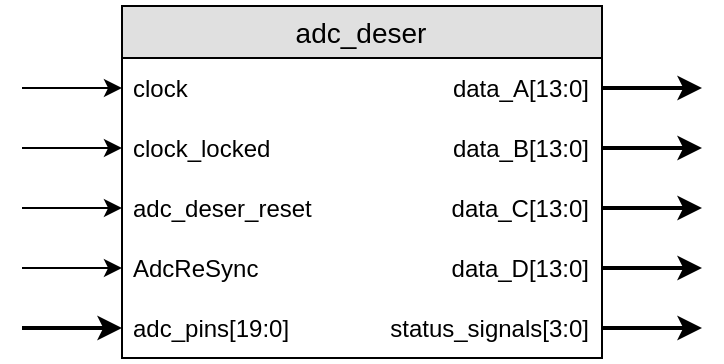
\includegraphics[width=0.5\linewidth]{adc_deser.png}
    \caption{Сигналы модуля десериализатора}
    \label{fig:mpr}
\end{figure}
Данный модуль был разработан ранее на основе готового интерфейса компании Xilinx, поэтому подробного описания его работы приведено не будет. Стоит лишь отметить, что входные данные принимаются через набор сигналов adc\_pins, а десериализованные значения подаются на выход через сигналы data\_i.\par
\textbf{ФАПЧ infrastructure\_top}\par
Модуль фазовой автоподстройки частоты (ФАПЧ) необходим для генерации тактового сигнала для работы АЦП и блоков, которые занимаются обработкой входных данных и их буферизацией (модули десериализатора и блока буферов). Как и десериализатор модуль ФАПЧ был разработан ранее с использованием библиотеки сложных функциональных блоков и рассматриваться подробно не будет. Сигналы модуля infrastructure\_top, в котором расположен ФАПЧ изображены на рисунке().\par
\begin{figure}[ht]
    \centering
    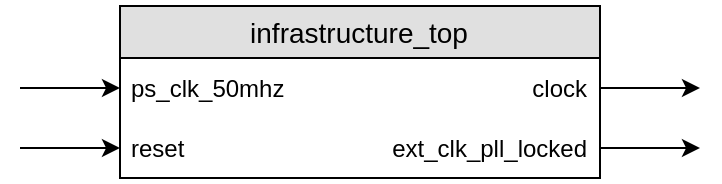
\includegraphics[width=0.5\linewidth]{infrastructure_top.png}
    \caption{Сигналы модуля infrastructure\_top}
    \label{fig:mpr}
\end{figure}
\textbf{Блок буферов buffers\_block}\par

